% Asset ID: A22StatisticalHypothesisTestingTikZ-004
% Source: Chapter 7 Hypothesis Testing Binomial transcript
% Related lesson section: Two-tailed critical regions
% Purpose: Show two-tailed critical regions.
% Related LO IDs: A22-HT-LO001, A22-HT-LO002, A22-HT-LO003

\documentclass[tikz,border=8pt]{standalone}
\usepackage{amsmath}
\usetikzlibrary{arrows.meta, positioning, decorations.pathreplacing}
\begin{document}
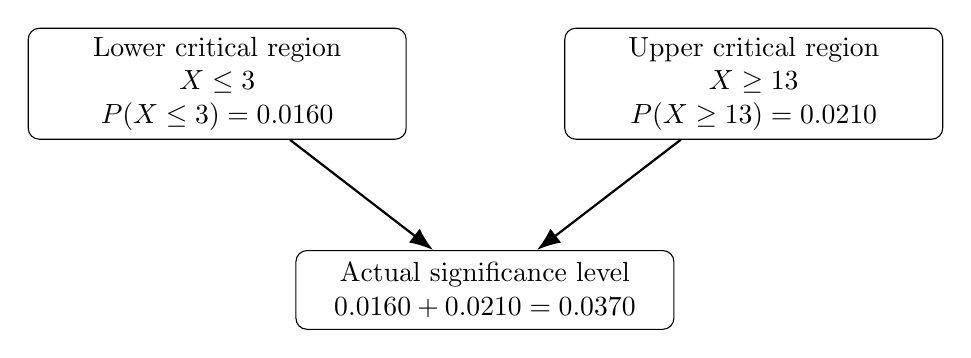
\begin{tikzpicture}[node distance=1.2cm, box/.style={draw, rounded corners, align=center, minimum width=4.8cm, minimum height=1.0cm}, arrow/.style={-{Latex[length=3mm]}, thick}]

\node[box] (low) {Lower critical region\\\(X\leq 3\)\\\(P(X\leq3)=0.0160\)};
\node[box, right=2cm of low] (high) {Upper critical region\\\(X\geq 13\)\\\(P(X\geq13)=0.0210\)};
\node[box, below=1.4cm of low, xshift=3.4cm] (actual) {Actual significance level\\\(0.0160+0.0210=0.0370\)};
\draw[arrow](low)--(actual);\draw[arrow](high)--(actual);

\end{tikzpicture}
\end{document}
